\documentclass[journal,12pt,twocolumn]{IEEEtran}

\usepackage{setspace}
\usepackage{gensymb}

\singlespacing


\usepackage[cmex10]{amsmath}

\usepackage{amsthm}

\usepackage{mathrsfs}
\usepackage{txfonts}
\usepackage{stfloats}
\usepackage{bm}
\usepackage{cite}
\usepackage{cases}
\usepackage{subfig}

\usepackage{longtable}
\usepackage{multirow}

\usepackage{enumitem}
\usepackage{mathtools}
%\usepackage{steinmetz}
\usepackage{tikz}
\usepackage{circuitikz}
\usepackage{verbatim}
%\usepackage{tfrupee}
\usepackage[breaklinks=true]{hyperref}

\usepackage{tkz-euclide}

\usetikzlibrary{calc,math}
\usepackage{listings}
    \usepackage{color}                                            %%
    \usepackage{array}                                            %%
    \usepackage{longtable}                                        %%
    \usepackage{calc}                                             %%
    \usepackage{multirow}                                         %%
    \usepackage{hhline}                                           %%
    \usepackage{ifthen}                                           %%
    \usepackage{lscape}     
\usepackage{multicol}
\usepackage{chngcntr}

\DeclareMathOperator*{\Res}{Res}

\renewcommand\thesection{\arabic{section}}
\renewcommand\thesubsection{\thesection.\arabic{subsection}}
\renewcommand\thesubsubsection{\thesubsection.\arabic{subsubsection}}

\renewcommand\thesectiondis{\arabic{section}}
\renewcommand\thesubsectiondis{\thesectiondis.\arabic{subsection}}
\renewcommand\thesubsubsectiondis{\thesubsectiondis.\arabic{subsubsection}}


\hyphenation{op-tical net-works semi-conduc-tor}
\def\inputGnumericTable{}                                 %%

\lstset{
%language=C,
frame=single, 
breaklines=true,
columns=fullflexible
}
\begin{document}


\newtheorem{theorem}{Theorem}[section]
\newtheorem{problem}{Problem}
\newtheorem{proposition}{Proposition}[section]
\newtheorem{lemma}{Lemma}[section]
\newtheorem{corollary}[theorem]{Corollary}
\newtheorem{example}{Example}[section]
\newtheorem{definition}[problem]{Definition}

\newcommand{\BEQA}{\begin{eqnarray}}
\newcommand{\EEQA}{\end{eqnarray}}
\newcommand{\define}{\stackrel{\triangle}{=}}
\bibliographystyle{IEEEtran}
\providecommand{\mbf}{\mathbf}
\providecommand{\pr}[1]{\ensuremath{\Pr\left(#1\right)}}
\providecommand{\qfunc}[1]{\ensuremath{Q\left(#1\right)}}
\providecommand{\sbrak}[1]{\ensuremath{{}\left[#1\right]}}
\providecommand{\lsbrak}[1]{\ensuremath{{}\left[#1\right.}}
\providecommand{\rsbrak}[1]{\ensuremath{{}\left.#1\right]}}
\providecommand{\brak}[1]{\ensuremath{\left(#1\right)}}
\providecommand{\lbrak}[1]{\ensuremath{\left(#1\right.}}
\providecommand{\rbrak}[1]{\ensuremath{\left.#1\right)}}
\providecommand{\cbrak}[1]{\ensuremath{\left\{#1\right\}}}
\providecommand{\lcbrak}[1]{\ensuremath{\left\{#1\right.}}
\providecommand{\rcbrak}[1]{\ensuremath{\left.#1\right\}}}
\theoremstyle{remark}
\newtheorem{rem}{Remark}
\newcommand{\sgn}{\mathop{\mathrm{sgn}}}
\providecommand{\abs}[1]{\left\vert#1\right\vert}
\providecommand{\res}[1]{\Res\displaylimits_{#1}} 
\providecommand{\norm}[1]{\left\lVert#1\right\rVert}
%\providecommand{\norm}[1]{\lVert#1\rVert}
\providecommand{\mtx}[1]{\mathbf{#1}}
\providecommand{\mean}[1]{E\left[ #1 \right]}
\providecommand{\fourier}{\overset{\mathcal{F}}{ \rightleftharpoons}}
%\providecommand{\hilbert}{\overset{\mathcal{H}}{ \rightleftharpoons}}
\providecommand{\system}{\overset{\mathcal{H}}{ \longleftrightarrow}}
	%\newcommand{\solution}[2]{\textbf{Solution:}{#1}}
\newcommand{\solution}{\noindent \textbf{Solution: }}
\newcommand{\cosec}{\,\text{cosec}\,}
\providecommand{\dec}[2]{\ensuremath{\overset{#1}{\underset{#2}{\gtrless}}}}
\newcommand{\myvec}[1]{\ensuremath{\begin{pmatrix}#1\end{pmatrix}}}
\newcommand{\mydet}[1]{\ensuremath{\begin{vmatrix}#1\end{vmatrix}}}
\numberwithin{equation}{subsection}
\makeatletter
\@addtoreset{figure}{problem}
\makeatother
\let\StandardTheFigure\thefigure
\let\vec\mathbf
\renewcommand{\thefigure}{\theproblem}
\def\putbox#1#2#3{\makebox[0in][l]{\makebox[#1][l]{}\raisebox{\baselineskip}[0in][0in]{\raisebox{#2}[0in][0in]{#3}}}}
     \def\rightbox#1{\makebox[0in][r]{#1}}
     \def\centbox#1{\makebox[0in]{#1}}
     \def\topbox#1{\raisebox{-\baselineskip}[0in][0in]{#1}}
     \def\midbox#1{\raisebox{-0.5\baselineskip}[0in][0in]{#1}}
\vspace{3cm}
\title{EE5609 Assignment 1}
\author{SHANTANU YADAV }
\maketitle
\newpage
\bigskip
\renewcommand{\thefigure}{\theenumi}
\renewcommand{\thetable}{\theenumi}

The python solution code is available at
\begin{lstlisting}
       https://github.com/Shantanu2508/assignment-1/blob/master/stline.py
\end{lstlisting}
%
and latex codes from 
\begin{lstlisting}
https://github.com/Shantanu2508/assignment-1/blob/master/assignment1.tex
\end{lstlisting}
%
\section{Problem}
Find the equations of the lines which intercepts on the both the axes and whose
	sum and product are 1 and -6 respectively.

\section{Solution}
	The equation of line in terms of vector notations can be written as
\begin{align}
	\vec{n}^T \vec{x} = c  
\end{align}
Let the intercepts be $\myvec{a \\ 0}$ and $\myvec{0 \\ b}$, respectively.

	Given that: \quad $ a + b = 1 $, \quad and \quad $ ab = -6$ 

The quadratic equation whose roots are the x and y intercepts can be written as:
\begin{align}
	x^2 - (\text{sum of roots})x &+ (\text{product of roots}) = 0 \\
	\implies \qquad & x^2 - x -6 =0 \\
	\implies \qquad & x=(3,-2) 
\end{align}
and corresponding $y$ intercepts are $(-2,3)$. 

The line $L_1$ passes through $\myvec{3 \\ 0}$ and $\myvec{0 \\ -2}$.

%.............................................................................
Let direction vector of this line be $\vec{m}$.
\begin{align}
	\vec{m} = \myvec{0\\-2} - \myvec{3\\0} = \myvec{-3\\-2}
\end{align}
The normal vector, $\vec{n}$: 
\begin{align}
	{\vec{n}} = \myvec{0 & -1 \\ 1 & 0}\vec{m} = \myvec{2 \\ -3}
\end{align}
%.............................................................................
The equation of line in terms of normal vector and passing through a point $A$ 
	is
\begin{align}
	\quad \vec{n^T}(\vec{x} - A ) = 0
	\quad \implies \quad \vec{n^Tx} = \vec{n^T}A \\
	\implies \vec{n^Tx}= \myvec{2 -3}\myvec{3 \\ 0} \\
	\implies \myvec{2 -3}\vec{x} = 6	\label{eqL1}
\end{align}
Similarly, the equation of second line $L_2$, with $x$ and 
	$y$ intercepts $\myvec{ -2 \\ 0}$ and $\myvec{ 0 \\ 3}$ and 
	normal vector $\myvec{ -3 \\ 2}$ is
\begin{align}
	\myvec{-3 &  2 } {\vec{x}} = 6	\label{eqL2}
\end{align}
The equations of lines (\ref{eqL1}) and (\ref{eqL2}) can be represented 
	collectively as
\begin{align}
	\myvec{2 & -3 \\ -3 & 2}\vec{x} = \myvec{6 \\ 6}
\end{align}

%.............................................................................
\begin{table}[htbp]
	\centering
	\begin{tabular}{|c|c|c|} \hline 
	$x-$intercept & $y-$intercept & \quad $\vec{n}$  \\ \hline \hline
	\myvec{3\\0}	&	\myvec{0\\-2}	&	\myvec{2\\-3} \\ \hline
	\myvec{-2\\0}	&	\myvec{0\\3}	&	\myvec{-3\\2} \\ \hline
	\end{tabular}
	\caption{} \label{coeftable}
\end{table}
%.............................................................................
\begin{figure}[!h]
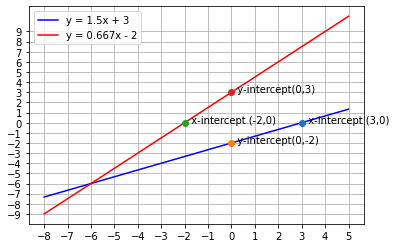
\includegraphics[width=\columnwidth]{stline_plot.png}
	\caption{}  \label{linefig1} 
\end{figure}

\end{document}
